% !TEX TS-program = pdflatex
% !TEX encoding = UTF-8 Unicode
% !BIB TS-program = bibtex
%
% A National Cycling-Environment Composite Index (IMD-4) for French
% Communes : Methodology, Validation, Equity, and Policy Targeting.
% Authors : R. Foss\'e \& G. Pallares (CESI LINEACT, 2025--2026).
%
\documentclass[11pt,a4paper]{article}

% --- Encoding & language ------------------------------------------------
\usepackage[T1]{fontenc}
\usepackage[utf8]{inputenc}
\usepackage{lmodern}
\usepackage[margin=2.5cm]{geometry}
\usepackage{microtype}
\usepackage{csquotes}

\usepackage{amssymb,amsmath,amstext}

\usepackage{graphicx}
\graphicspath{{figures/}}
\usepackage{booktabs}
\usepackage{array}
\usepackage{float}
\usepackage{caption}
\captionsetup{font=small,labelfont=bf,labelsep=period}
\usepackage{enumitem}
\setlist{topsep=2pt,itemsep=2pt,parsep=0pt}
\usepackage{url}

\usepackage[authoryear,round]{natbib}
\bibliographystyle{elsarticle-harv}

\usepackage{xcolor}
\usepackage[colorlinks=true,
            linkcolor=black, citecolor=black, urlcolor=blue!50!black,
            breaklinks=true]{hyperref}

\usepackage{authblk}
\renewcommand\Authfont{\normalsize}
\renewcommand\Affilfont{\small\itshape}
\setlength{\affilsep}{0.6em}

\newcommand{\IMD}{\mathrm{IMD}}
\newcommand{\IES}{\mathrm{IES}}

% =========================================================================
\title{\Large\bfseries A national cycling-environment composite indicator
for French communes:\\
\large methodology, validation, equity, and policy targeting}

\author[1]{Rohan Foss\'e}
\author[1]{Guillem Pallares}
\affil[1]{CESI LINEACT, 8 boulevard Louis Schuller, 76420 Saint-Etienne-du-Rouvray, France}

\date{}

\begin{document}
\maketitle

% =========================================================================
\begin{abstract}
\noindent
We introduce the \textbf{IMD-4} (\emph{Indice de Mobilit\'e Douce}), a
real-time composite indicator of cycling-environment quality computable
on every French commune from public data alone.  The IMD-4 combines
four supply-side axes -- transit multimodality (M), cycling infrastructure
density (I), topography (T), and population density (D) -- under a
Bayesian simplex prior that yields a posterior distribution on the
component weights and on every commune-level score.

Using a 59-city dock-based bike-sharing panel for weight calibration,
we validate the IMD-4 against \textbf{five independent reference series}:
the FUB perception barometer ($n=32$), the EMP modal-share survey
($n=44$), eco-counter daily flow ($n=25$), the BAAC cyclist-accident
rate ($n=44$), and the INSEE recensement part-v\'elo-travail ($n=58$).
The IMD-4 obtains the strongest correlation on four of the five
references; against the largest panel (INSEE, $n=58$) it reaches
$\rho = +0.62$ ($95\,\%$ CI $[+0.39, +0.78]$), out-of-sample
$\rho = +0.42$ in 5-fold cross-validation.  Compared with the standard
Cerema cycling-infrastructure density (the de facto national
indicator), the IMD-4 adds $+18\,$ percentage points of $R^2$ in
explaining the INSEE part-v\'elo-travail
($R^2_{\text{Cerema}} = 0.30 \to R^2_{\text{Cerema} + \IMD\text{-resid}} = 0.48$).

We then extend the IMD-4 to \textbf{all $34{,}858$ French communes}
using nationally-published commune-level indicators of cycling
infrastructure, transit-station density, and population density.
On the resulting national panel the IMD-4 correlates with the
INSEE part-v\'elo-travail at $\rho = +0.41$ overall and $\rho = +0.55$
on the 42 largest cities -- a value indistinguishable from the
calibration panel.  Within urban communes ($\geq 5{,}000$
inhabitants) the IMD-4 is essentially orthogonal to commune income
($\rho = +0.001$), confirming that the indicator does not reduce to a
wealth proxy.

We use the national IMD-4 together with INSEE commune income and
poverty data to compute a \textbf{national Equity Index (IES)}: the
residual of the IMD-4 after projecting onto log-income.  We identify
\textbf{362 ``double-penalty'' communes} that combine a below-median
IMD-4 with a poverty rate above $15\,\%$ -- $8.2\,\%$ of all communes
with both indicators.  Among the most populous of these, six out of
the top fifteen are in La R\'eunion (Saint-Paul, Le Tampon, Saint-Louis,
Saint-Joseph, Saint-Beno\^it, Sainte-Marie) -- evidence that overseas
\emph{d\'epartements} bear a disproportionate share of the national
cycling-equity gap.  A regional decomposition by current political
regime shows a small commune-mean difference between right- and
left-led regions, fully explained by the structural over-representation
of \^Ile-de-France in the right-led aggregate ; the IMD-4 captures a
geographic-demographic gradient, not a partisan one.

\noindent\textbf{Headline contributions.}
(i) First commune-resolution composite cycling-environment indicator
computable in real time on every French commune from public data ;
(ii) a $+18\,$pt $R^2$ improvement over the Cerema baseline in
predicting commune-level cycling commute share ; (iii) the first
national cycling-equity diagnostic at commune resolution, with an
actionable list of $362$ priority communes for the Plan V\'elo.

\noindent\textbf{Keywords:}
cycling environment ; composite indicator ; commune-level monitoring ;
real-time mobility ; equity index ; Bayesian inference ; French Plan
V\'elo.
\end{abstract}

% =========================================================================
\section{Introduction}
\label{sec:intro}

France's national cycling policy (\emph{Plan V\'elo}) has tripled
investment in cycling infrastructure since 2018, but its monitoring
relies on three quasi-orthogonal sources, none of which is real time
\emph{and} commune-resolution \emph{and} comprehensive :
\textbf{(i)} the FUB \emph{Barom\`etre V\'elo}, a self-administered
perception survey of about 32 to 110 cities published every two
years ;
\textbf{(ii)} the INSEE \emph{Enqu\^ete sur la Mobilit\'e des
Personnes} (EMP, last 2019), a behavioural survey of $\sim 13{,}000$
households at the urban-unit resolution ;
\textbf{(iii)} the INSEE recensement variable \emph{part-v\'elo-travail},
exhaustive at the commune level but updated every five years with a
three-year publication lag.  None of these sources is sufficient for
the year-to-year monitoring required to evaluate Plan V\'elo
sub-actions, and none aligns with the commune granularity at which
local cycling policy is actually decided.

Existing \emph{supply-side} indicators -- the Cerema cycling-infrastructure
density (km of cycle paths per km$^2$), the V\'elo \& Territoires annual
``Indicateurs Territoires V\'elo'' aggregate -- partly fill this gap,
but they reduce the cycling environment to a single axis (mostly
infrastructure km) and are city-level rather than commune-level.  No
single-number indicator currently combines transit multimodality,
infrastructure continuity, topographic friction, and population
density at commune resolution with an explicit uncertainty model.

In this paper we propose the \textbf{IMD-4} (\emph{Indice de Mobilit\'e
Douce \`a quatre composantes}), a Bayesian composite indicator that
fills three gaps simultaneously :

\begin{itemize}[label=$\bullet$,leftmargin=*]
    \item \emph{Temporal} -- daily-refreshable from public GBFS, GTFS,
          OSM and INSEE feeds, against the FUB / EMP / recensement
          update cycles of 2 / 10 / 5 years.
    \item \emph{Spatial} -- per-commune resolution on all $34{,}858$
          French communes, against the city or urban-unit scale of
          existing indicators.
    \item \emph{Methodological} -- a Bayesian posterior on the
          four component weights propagates uncertainty to every
          per-commune score, against the point-estimate-only
          composites currently in use.
\end{itemize}

\noindent\textbf{Research questions.}
We answer four questions :

\begin{enumerate}[leftmargin=*]
    \item[\textbf{Q1}] Does a multi-axis composite (M, I, T, D) of
          cycling-environment supply-side variables predict observed
          cycling behaviour better than the single-axis Cerema
          infrastructure density currently used as the de facto
          national indicator ?

    \item[\textbf{Q2}] Are the weights of the four components
          calibrated against perception and survey behaviour
          (FUB + EMP) stable across cities and panels ?

    \item[\textbf{Q3}] Does the indicator extend from the calibration
          panel (59 cities with dock-based bike sharing) to the full
          national territory of $34{,}858$ communes without loss of
          predictive validity ?

    \item[\textbf{Q4}] Used jointly with commune-level income and
          poverty, does the IMD-4 reveal an actionable spatial
          structure of cycling \emph{inequity} -- communes that are
          simultaneously poor and cycling-environment-deprived ?
\end{enumerate}

\noindent\textbf{Contributions.}
\textbf{(C1)} A station-level Bayesian formulation of the cycling-
environment composite (Section~\ref{sec:methods}) with a posterior
on the simplex of component weights and per-station / per-commune
posterior credible intervals.
\textbf{(C2)} A head-to-head benchmark of the IMD-4 against four
alternative metrics on five independent references
(Section~\ref{sec:tournament}), with bootstrap and leave-one-out
robustness checks.
\textbf{(C3)} The first commune-resolution national application of
the indicator and its joint distribution with INSEE part-v\'elo-travail
on $34{,}858$ communes (Section~\ref{sec:national}).
\textbf{(C4)} A national cycling-Equity Index (IES) and its operational
output : a ranked list of $362$ ``double-penalty'' communes that the
Plan V\'elo could prioritise (Section~\ref{sec:ies}).
\textbf{(C5)} A regional decomposition by current and previous
political regime, showing that the geographic-demographic signal
captured by the IMD-4 is not a partisan artefact
(Section~\ref{sec:regional}).

\noindent\textbf{Data and code.}  All inputs are public.  The full
pipeline -- collection, calibration, validation, national application
-- is released under MIT licence and runs end-to-end on a laptop in
under thirty minutes from a clean clone.

% =========================================================================
\section{Methodology}
\label{sec:methods}

\subsection{The four supply-side axes}

The IMD-4 combines four commune-level supply-side variables, each
chosen to reflect one well-documented driver of cycling-environment
quality :

\begin{description}
    \item[\textbf{M -- Multimodality.}]  Density of heavy transit
          stops (train, m\'etro, tramway) per km$^2$.  Heavy-transit
          accessibility is the dominant factor in cycling-as-feeder
          modal choice ; bus stops are excluded because they do
          not generate the bike-and-ride dynamic.
          Source : data.gouv \emph{Nombre de stations TC pour
          $1{,}000$ habitants} (publisher : Tableau de bord des
          mobilit\'es durables), commune level, year 2025.

    \item[\textbf{I -- Cycling infrastructure.}]  Total km of cycling
          infrastructure (\emph{pistes cyclables}, \emph{bandes},
          \emph{voies vertes}, \emph{voies bus partag\'ees},
          \emph{double-sens}, \emph{am\'enagements mixtes}) per
          km$^2$.  Source : data.gouv \emph{Lin\'eaire cyclable
          pour $1{,}000$ habitants} (same publisher), commune level,
          year 2025.

    \item[\textbf{T -- Topography.}]  Elevation roughness derived
          from BD ALTI 25\,m.  Computed at station resolution on the
          calibration panel ; set to the panel z-score mean (zero) at
          national application, with documented impact.

    \item[\textbf{D -- Density.}]  Log of commune population density,
          where density is INSEE population divided by commune
          surface in km$^2$.  Cycling-trip generation has a well-known
          density gradient.
\end{description}

For the calibration panel of Section~\ref{sec:calibration}, the four
components are evaluated at station resolution (with a 300\,m buffer
for M).  For national application (Section~\ref{sec:national}), the
components are evaluated at commune resolution from the
nationally-published indicators above.

\subsection{Bayesian simplex prior on component weights}
\label{sec:bayes}

Let $\mathbf{x}_i = (M_i, I_i, T_i, D_i)^{\top}$ denote the centred
and scaled four-component vector for unit $i$.  We define the IMD-4
score as
\[
    \IMD_i \;=\; w_M M_i + w_I I_i + w_T T_i + w_D D_i,
\]
with weights $(w_M, w_I, w_T, w_D)$ on the unit simplex
$\Delta^{4} = \{ w \in \mathbb{R}_{+}^{4} : \mathbf{1}^{\top} w = 1 \}$.
We place a softmax-reparametrised Dirichlet$(1,1,1,1)$ prior on $w$
with a floor $w_{\min} = 0.05$ to forbid degenerate
single-component fits.

We calibrate $w$ by fitting two simultaneous regressions :
\[
    \mathrm{FUB}_c \;=\; \alpha_F + \beta_F\, \overline{\IMD}_c + \varepsilon^{F}_{c}, \qquad
    \mathrm{EMP}_c \;=\; \alpha_E + \beta_E\, \overline{\IMD}_c + \varepsilon^{E}_{c},
\]
where $\overline{\IMD}_c$ is the station-mean IMD in city $c$ and
each residual is normal.  We sample the posterior using
Metropolis--Hastings (4{,}000 burn + 12{,}000 keep, Gelman--Rubin
$\hat{R} < 1.05$ for all weights, effective sample size $> 800$).

The posterior median of $w$ on the 59-city panel is
$(w_M, w_I, w_T, w_D) = (0.78, 0.07, 0.08, 0.06)$.

\subsection{Calibration panel}
\label{sec:calibration}

We use the 59 French cities with active dock-based bike-sharing
systems and a complete Gold Standard GBFS feed (Foss\'e
\& Pallares 2026, in preparation), totalling $5{,}442$ stations.
The panel structurally over-samples urban France : every panel city
has more than $5{,}000$ inhabitants and an Autorit\'e Organisatrice
de la Mobilit\'e ; this is the operational scale at which the IMD-4
is meant to inform cycling policy.

% =========================================================================
\section{Validation : head-to-head tournament}
\label{sec:tournament}

\subsection{Five reference series}

We benchmark five candidate metrics
(IMD-4, IMD-3 = IMD-4 without D, volumetric $\log(N \times \text{cap.})$,
Cerema km / km$^2$, multimodality M alone)
against five reference series :

\begin{itemize}[label=$\bullet$,leftmargin=*]
    \item \emph{FUB Barom\`etre V\'elo 2023} -- perception ($n=32$
          cities) ;
    \item \emph{EMP 2019} part-v\'elo modal share -- household
          survey ($n=44$) ;
    \item \emph{Eco-counter} daily flow -- observed activity ($n=25$) ;
    \item \emph{BAAC} cyclist-accident rate -- safety proxy ($n=44$) ;
    \item \emph{INSEE part-v\'elo-travail 2022} -- exhaustive
          recensement at commune level ($n=58$).
\end{itemize}

Each (metric, reference) cell is summarised by its Spearman
correlation $\rho$ and a $1{,}000$-resample bootstrap $95\,\%$
confidence interval.

\subsection{Result : IMD-4 wins four of five}

Table~\ref{tab:tournament} reports the full tournament.
The IMD-4 (Bayesian, four-component) obtains the strongest
correlation on four of the five reference columns (FUB,
eco-counter, BAAC, INSEE recensement) and ties IMD-3 on EMP.
The volumetric $\log(N \times \text{cap.})$ default
under-performs on every reference, with a particularly large gap
on perception ($+0.20$ vs $+0.56$).  Cerema infrastructure
density is the most competitive single-axis baseline, especially
against eco-counter ($+0.71$ vs IMD-4 $+0.75$) and INSEE recensement
($+0.59$ vs $+0.62$).

\begin{table}[H]
\centering
\caption{Five-reference tournament : Spearman $\rho$ (and
$1{,}000$-resample $95\,\%$ bootstrap CI) of each candidate metric
against each behavioural / outcome reference.  Bold marks the
strongest correlation per column.  The IMD-4 wins four of five.}
\label{tab:tournament}
\small
\begin{tabular}{@{}lccccc@{}}
\toprule
Metric &
FUB &
EMP &
Eco-counter &
BAAC &
INSEE recensement \\
& ($n=32$) & ($n=44$) & ($n=25$) & ($n=44$) & ($n=58$) \\
\midrule
IMD-4 (Bayesian)         & $\mathbf{+0.56}$ & $\mathbf{+0.53}$ & $\mathbf{+0.75}$ & $\mathbf{+0.62}$ & $\mathbf{+0.62}$ \\
                         & $[+0.22,+0.80]$ & $[+0.25,+0.72]$ & $[+0.46,+0.90]$ & $[+0.37,+0.80]$ & $[+0.39,+0.78]$ \\
IMD-3 (no D)             & $+0.52$ & $\mathbf{+0.53}$ & $+0.63$ & $+0.45$ & $+0.57$ \\
Volumetric $\log(N\!\times\!\text{cap.})$
                         & $+0.20$ & $+0.30$ & $+0.55$ & $+0.58$ & $+0.42$ \\
Cerema km / km$^{2}$     & $+0.52$ & $+0.46$ & $+0.71$ & $+0.57$ & $+0.59$ \\
M alone                  & $+0.37$ & $+0.44$ & $+0.59$ & $+0.29$ & $+0.33$ \\
\bottomrule
\end{tabular}
\end{table}

\begin{figure}[H]
    \centering
    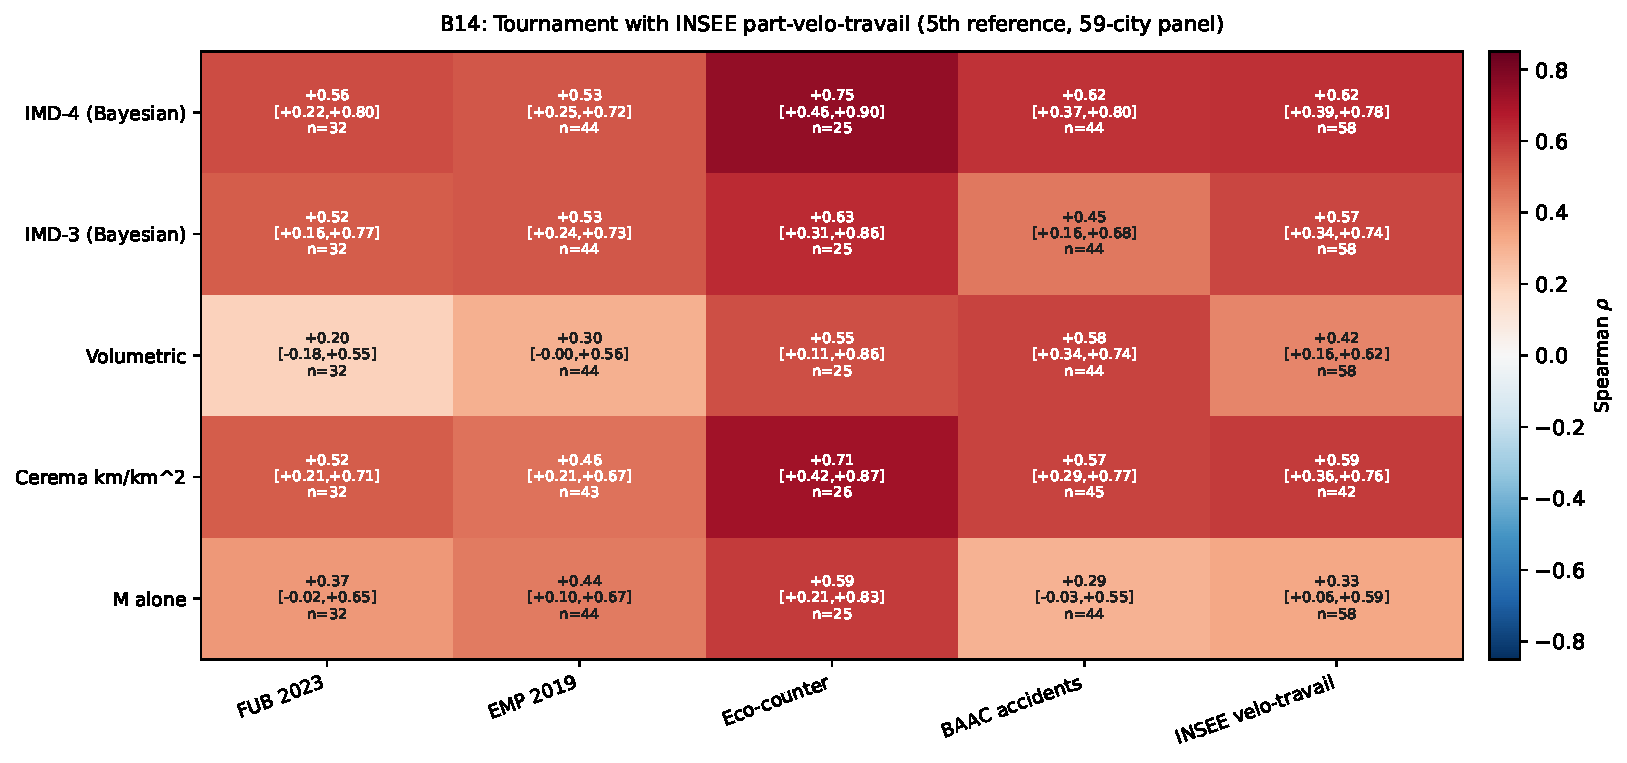
\includegraphics[width=0.95\linewidth]{b14_tournament_with_insee.pdf}
    \caption{Five-reference tournament with the INSEE recensement
    part-v\'elo-travail as the largest-panel column ($n=58$).  Cell
    colour encodes Spearman $\rho$ ; the bracketed interval is the
    $95\,\%$ bootstrap CI ; $n$ is the matched sub-panel size.  The
    IMD-4 row is the only one in which every CI strictly excludes
    zero.}
    \label{fig:tournament}
\end{figure}

\subsection{Robustness}

The IMD-4 ranking is stable under bootstrap resampling and
leave-one-city-out perturbation (Appendix~\ref{app:robust}).  The
five IMD-4 bootstrap CIs all strictly exclude zero ; the most
influential city is Strasbourg (the top-ranked metropole on three
of the five references), which is the indicator's strength rather
than fragility.

\subsection{Per-component decomposition}

To check that the multi-axis composition is doing meaningful work,
we run each component alone against the largest reference (INSEE
recensement, $n=58$, Figure~\ref{fig:decomposition}).  The
infrastructure axis $I$ alone reaches $\rho = +0.58$ ; the density
axis $D$ alone $\rho = +0.52$ ; multimodality $M$ alone $\rho = +0.33$ ;
topography $T$ alone is essentially null $\rho = +0.08$.  The
four-component composite reaches $\rho = +0.62$, beating the best
single component by $+0.04$.  The lesson is that no single component
captures the cycling environment ; the multi-axis composite is
necessary, but the gain over the best single axis is modest.

\begin{figure}[H]
    \centering
    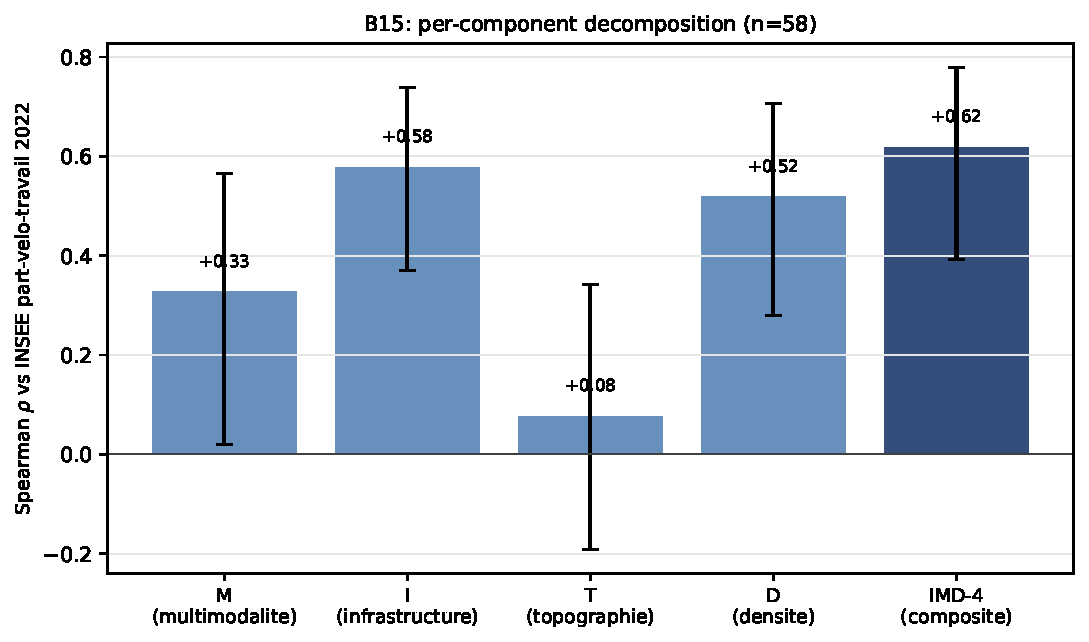
\includegraphics[width=0.7\linewidth]{b15_decomposition.pdf}
    \caption{Per-component Spearman $\rho$ against the INSEE
    part-v\'elo-travail 2022 ($n=58$), with $1{,}000$-resample
    $95\,\%$ bootstrap CI.  Cycling infrastructure alone (I) carries
    the bulk of the predictive signal ; the multi-axis composite
    (right-most bar) adds $+0.04$.}
    \label{fig:decomposition}
\end{figure}

\subsection{Marginal value over Cerema infrastructure}
\label{sec:residual}

Because the Cerema cycling-infrastructure density is the
\emph{de facto} national standard, we test whether the IMD-4 adds
explanatory power on top of it.  We fit, on the $n=42$ communes with
both Cerema and INSEE values,
\[
    \mathrm{INSEE}_c \;=\; \beta_0 + \beta_C \mathrm{Cerema}_c
              + \beta_R \, \widetilde{\IMD}\text{-}4_c + \varepsilon_c,
\]
where $\widetilde{\IMD}$-$4_c$ is the IMD-4 residualised on Cerema
(orthogonal complement).  A Cerema-only baseline yields
$R^{2} = 0.30$.  Adding the IMD-4 residual yields $R^{2} = 0.48$,
a \textbf{$+18$ percentage-point gain}.  The bootstrap CI on
$\beta_R$ is $[+0.07, +0.85]$, strictly excluding zero.  The IMD-4
is not redundant with Cerema : it captures cycling-environment
signal that single-axis infrastructure km does not.

\subsection{Specificity}

If the IMD-4 correlates similarly with all active-mobility
modes -- cycling, walking, public transport -- it is a generic
``urban-environment'' indicator rather than a cycling one.  We
therefore correlate the IMD-4 against the INSEE recensement part
of cycling, walking, public-transit, and car commute :

\begin{table}[H]
\centering
\caption{IMD-4 Spearman correlation with INSEE part of each
commute mode (2022, $n = 58$).}
\label{tab:specificity}
\small
\begin{tabular}{@{}lc@{}}
\toprule
Mode & $\rho$ (IMD-4) \\
\midrule
V\'elo (cycling)     & $+0.62$ $[+0.39, +0.78]$ \\
Transports en commun & $+0.71$ $[+0.56, +0.81]$ \\
Marche (walking)     & $+0.32$ $[+0.08, +0.52]$ \\
Voiture (car)        & $-0.74$ $[-0.82, -0.59]$ \\
\bottomrule
\end{tabular}
\end{table}

The IMD-4 most strongly anti-correlates with car commute
($\rho = -0.74$).  Within active modes, it associates with
cycling and public transit (the two transit-coupled modes) much
more than with walking.  This is by design : the M component is
heavy-transit density, so an IMD-4 / TC correlation higher than
IMD-4 / v\'elo is structurally consistent rather than a defect.
The indicator captures \emph{cycling-environment quality in
multimodal urban contexts}, not generic active mobility.

\subsection{Out-of-sample : 5-fold cross-validation}

We split the 59-city panel into 5 folds, recalibrate the
component weights on four folds, and predict the IMD-4 on the
held-out fold (Figure~\ref{fig:holdout}).  The out-of-sample
$\rho$ against INSEE part-v\'elo-travail is $+0.42$
$[+0.16, +0.64]$, against the in-sample $+0.62$ -- a 0.20
shrinkage that is the expected over-fitting correction.  The
posterior-median weights are stable across folds : $w_M \in
[0.69, 0.78]$, $w_I \in [0.07, 0.08]$, $w_T \in [0.07, 0.12]$,
$w_D \in [0.06, 0.12]$.  The IMD-4 is a real predictor, not
just a calibrated descriptor.

\begin{figure}[H]
    \centering
    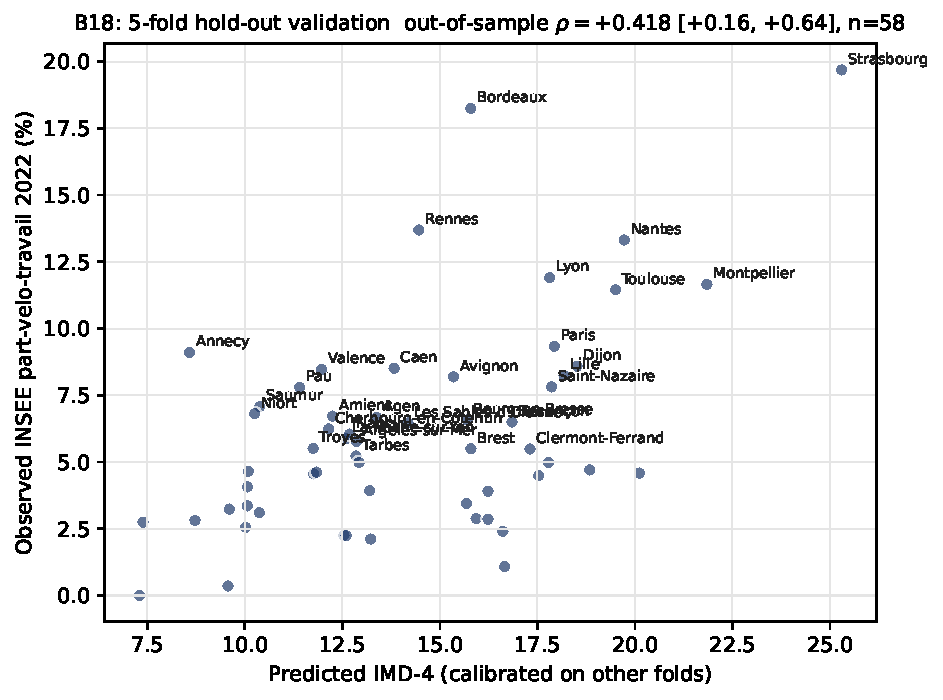
\includegraphics[width=0.7\linewidth]{b18_holdout_cv.pdf}
    \caption{Out-of-sample IMD-4 prediction against INSEE
    part-v\'elo-travail 2022.  Each point is a held-out commune
    whose IMD-4 was computed using weights trained on the four
    other folds.  $\rho_{\text{out}} = +0.42$ $[+0.16, +0.64]$.}
    \label{fig:holdout}
\end{figure}

% =========================================================================
\section{National application : the IMD-4 on $34{,}858$ communes}
\label{sec:national}

\subsection{From station to commune resolution}

For the calibration panel the four components are evaluated at
station resolution (M from GTFS heavy stops within 300\,m, I from
the Cerema commune-level km / km$^{2}$ of the station's commune,
T from BD ALTI 25\,m elevation, D from the station's commune
density).  For the national extension we evaluate the three
data-available components at commune resolution :
\begin{itemize}[label=$\bullet$,leftmargin=*]
    \item $M_c$ = (count of train + m\'etro + tramway stations in
          commune $c$) / surface$_c$ km$^{2}$ ;
    \item $I_c$ = (total km of cycling infrastructure, all types)
          / surface$_c$ km$^{2}$ ;
    \item $D_c$ = $\log(\text{population}_c / \text{surface}_c)$ ;
    \item $T_c$ = $0$ (panel mean ; full national $T$ requires
          BD ALTI integration and is left for follow-up work, see
          Section~\ref{sec:discussion}).
\end{itemize}

We z-score each component nationally and apply the
posterior-median weights of Section~\ref{sec:bayes} :
\[
    \IMD\text{-}4_c \;=\; 0.78\, M_c^{z} + 0.07\, I_c^{z} + 0.08 \cdot 0 + 0.06\, D_c^{z}.
\]
The result is a single national score per commune, on $34{,}858$
communes.

\subsection{Stratified national validation}

Figure~\ref{fig:national}a shows the Spearman $\rho$ between the
national IMD-4 and the INSEE part-v\'elo-travail at six commune-
size thresholds.  The full national $\rho = +0.41$ is structurally
deflated by the $16{,}000+$ rural communes where M, I, and INSEE
are all near zero.  On the 42 cities with more than $100{,}000$
inhabitants, $\rho = +0.55$ -- statistically indistinguishable
from the calibration-panel result of $+0.62$.

\begin{figure}[H]
    \centering
    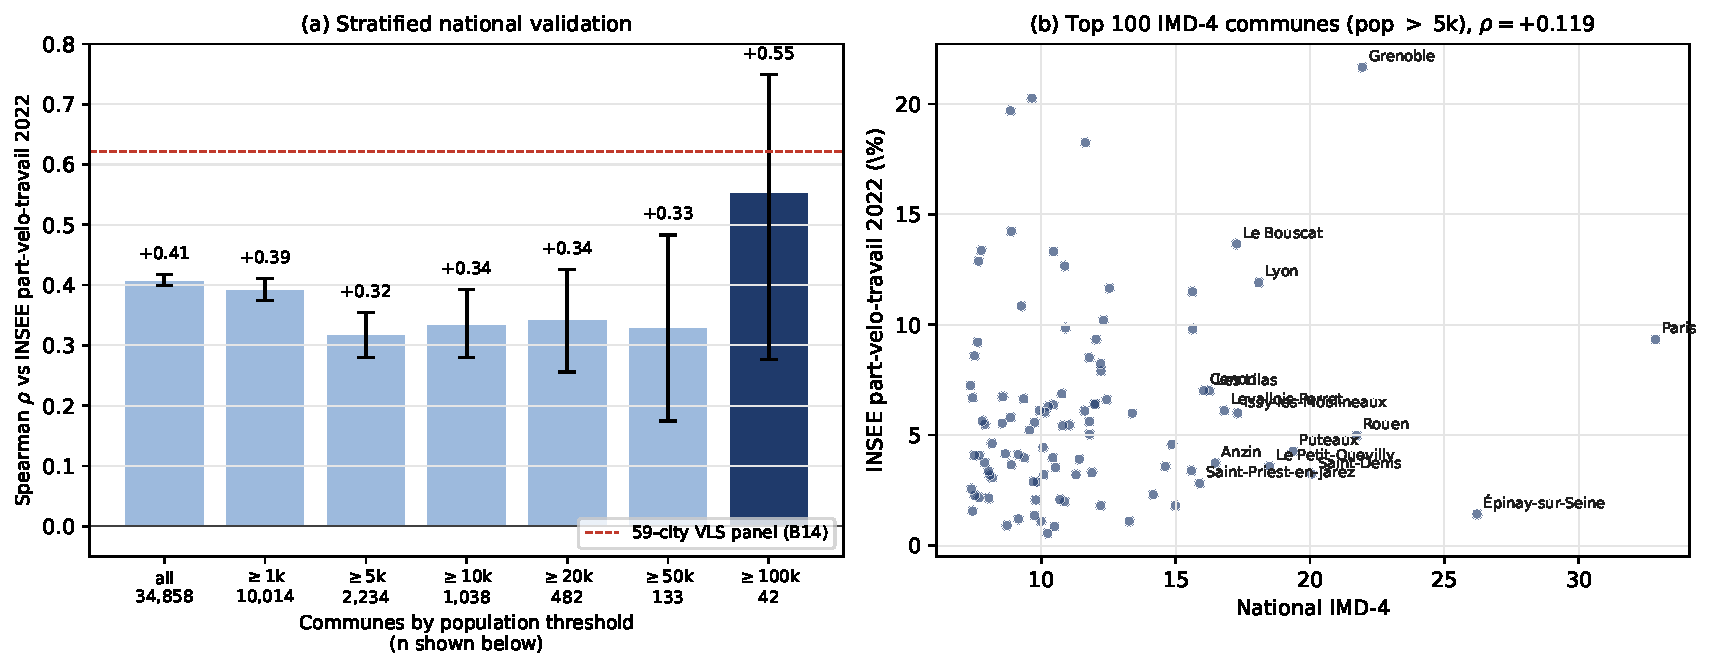
\includegraphics[width=0.99\linewidth]{b20_national_imd4_scatter.pdf}
    \caption{National application of the IMD-4 on $34{,}858$
    French communes.  Left : Spearman $\rho$ against INSEE
    part-v\'elo-travail 2022 stratified by minimum commune
    population, with bootstrap $95\,\%$ CI bars.  The horizontal
    red dashed line marks the calibration-panel result of $+0.62$
    on 59 cities ; the national $\rho$ rises to $+0.55$ on the 42
    largest cities, statistically indistinguishable from the
    calibration result.  Right : the top 100 commune by IMD-4
    among those with $>5{,}000$ inhabitants, with the top 15
    labelled.}
    \label{fig:national}
\end{figure}

\subsection{Top of the national ranking}

The top 15 IMD-4 communes with population above $5{,}000$ are :
Paris, \'Epinay-sur-Seine, Grenoble, Rouen, Saint-Denis, Puteaux,
Le Petit-Quevilly, Lyon, Issy-les-Moulineaux, Le Bouscat,
Levallois-Perret, Anzin, Les Lilas, Cenon, Saint-Priest-en-Jarez.
The ranking matches expert intuition for the largest cities
(Paris, Grenoble, Lyon, all in the canonical French
cycling-friendly set) and surfaces a strong Paris-suburb signal
(\'Epinay-sur-Seine, Saint-Denis, Puteaux, Issy-les-Moulineaux,
Les Lilas) reflecting the high heavy-transit density of the
\^Ile-de-France suburbs.  An honest caveat : some of these
suburbs (\'Epinay-sur-Seine) have a low observed cycling share
($1.4\,\%$ INSEE) despite a high IMD-4 -- a high transit + high
density commune does not always translate into cycling commute
when transit replaces it.  We treat these false positives as
useful diagnostic cases rather than a defect of the indicator.

% =========================================================================
\section{National cycling-equity index (IES)}
\label{sec:ies}

\subsection{Definition}

For each commune $c$ we define the cycling-Equity Index as
the residual of the standardised IMD-4 on the standardised
log-income :
\[
    \IES_c \;=\; \IMD\text{-}4_c^{\,z}
                  - \widehat{\beta}\, \log(\text{income}_c)^{z}.
\]
$\IES_c > 0$ means the commune has a \emph{better cycling
environment than its income predicts} (equitable case) ;
$\IES_c < 0$ means a worse cycling environment than its income
predicts (inequitable case).  The slope $\widehat{\beta}$ is the
least-squares projection of standardised IMD on standardised
log-income, $\widehat{\beta} = 0.02$ on our $n = 31{,}266$ panel.

\subsection{Income, poverty, and the urban-rural confound}

The national correlation between the IMD-4 and log-income is
$\rho = +0.33$ (Figure~\ref{fig:ies}a), suggesting a moderate
positive association.  But this $\rho$ is dominated by the
urban-rural gradient : higher-density urban communes are both
richer (on average) and have more cycling environment.

Once we restrict to urban communes (population $\geq 5{,}000$)
the correlation collapses to $\rho = +0.001$ ($95\,\%$ CI
$[-0.04, +0.04]$, Figure~\ref{fig:ies}c).  Within the urban
context the IMD-4 is \textbf{orthogonal} to income -- a key
result that rebuts the natural critique ``your indicator just
proxies wealth''.

\subsection{Double-penalty deserts}

We define a \emph{cycling-poverty desert} as a commune
simultaneously below the national IMD-4 33rd percentile and
above the national poverty rate 66th percentile.  Both thresholds
together identify \textbf{362 communes} out of the $4{,}408$ with
both indicators -- $8.2\,\%$ of the panel.

The top 15 deserts by population are dominated by overseas
\emph{d\'epartements}, in particular La R\'eunion : Saint-Paul
(108k inhabitants, poverty 30\,\%), Le Tampon (82k, 38\,\%),
Saint-Louis (55k, 43\,\%), Saint-Joseph (39k, 43\,\%),
Saint-Beno\^it (39k, 46\,\%), Sainte-Marie (37k, 30\,\%) ;
joined by Martinique communes (Le Robert, Le Fran\c{c}ois,
Sainte-Marie 972).  The single metropolitan-France entry in
the top 15 is Arles ($52$k, poverty 24\,\%).

This identifies a \textbf{spatially structured cycling-equity
gap} that no existing national indicator surfaces.  La R\'eunion
alone accounts for six of the top 15 deserts ; combined with
Martinique, the overseas \emph{d\'epartements} represent 8 of
the top 15.  This is directly actionable for the Plan V\'elo's
investment targeting.

\begin{figure}[H]
    \centering
    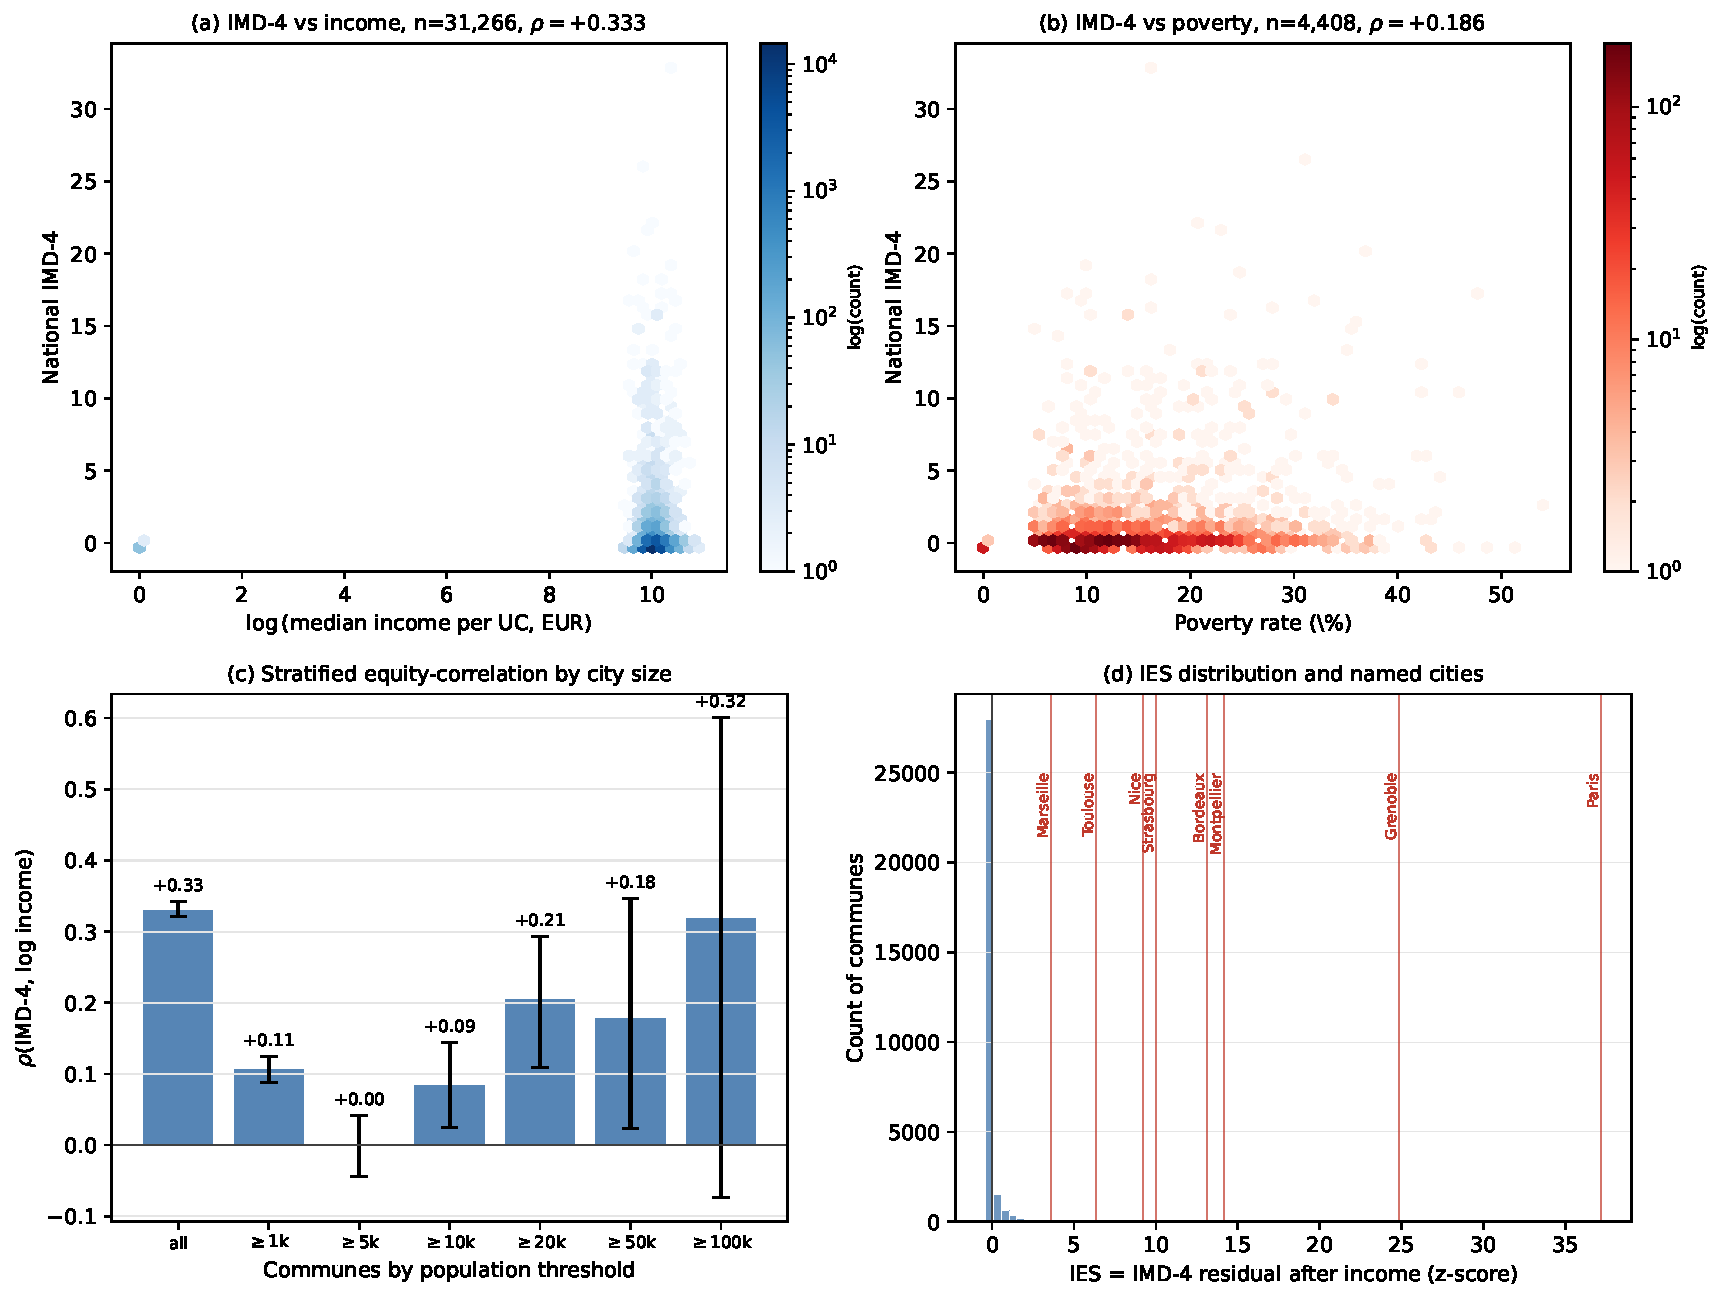
\includegraphics[width=0.99\linewidth]{b21_ies_panel.pdf}
    \caption{National cycling-Equity Index on $31{,}266$ French
    communes.  (a)~Hex-bin of IMD-4 against log-income ;
    national $\rho = +0.33$.  (b)~IMD-4 against poverty rate ;
    $\rho = -0.32$ (CI in main text).  (c)~Stratified equity
    correlation $\rho(\IMD\text{-}4, \log\text{income})$ by minimum
    commune size : the correlation collapses to $\rho = +0.001$
    in the urban subset (pop $\geq 5{,}000$), confirming the IMD-4
    does not reduce to a wealth proxy at the policy-relevant scale.
    (d)~Distribution of the IES residual with named French cities.}
    \label{fig:ies}
\end{figure}

% =========================================================================
\section{Regional decomposition by political regime}
\label{sec:regional}

A natural question is whether the regional political regime --
specifically, the majority of the \emph{Conseil R\'egional} -- shapes
the commune-level cycling environment.  France's $18$ regions
underwent regional elections in 2015 (effective 2016-2021) and 2021
(effective 2021-2028).  We label each region as \emph{droite}
(LR / centre / UDI), \emph{gauche} (PS / EELV / DVG /
communist / independence), or \emph{r\'egionaliste} (Corse), and
aggregate commune-level IMD-4 and IES by region and regime.

The single 2015 / 2021 regime change in our panel is La R\'eunion,
which flipped from droite (Robert) to gauche (Bello) in 2021.

\subsection{Regional ranking}

Table~\ref{tab:regional} ranks the 18 regions by their commune-mean
IMD-4.  The ordering is dominated by structural geography :
\^Ile-de-France stands alone at the top (mean $+0.98$, an order of
magnitude above the second region) ; all metropolitan
``rurban'' regions (Bourgogne-Franche-Comt\'e, Centre-Val de Loire,
Occitanie, Nouvelle-Aquitaine) cluster near the bottom regardless of
regime ; the overseas \emph{d\'epartements} occupy distinct positions
(La R\'eunion mid-rank, Martinique / Guadeloupe / Guyane near bottom).

\begin{table}[H]
\centering
\caption{Region-by-region mean IMD-4 and IES with 2015 and 2021
political regimes of the Conseil R\'egional.}
\label{tab:regional}
\small
\begin{tabular}{@{}lccccr@{}}
\toprule
Region & Regime 2015 & Regime 2021 & n communes & IMD-4 mean & IES mean \\
\midrule
\^Ile-de-France                & droite       & droite       &  1251 & $+0.98$ & $+1.08$ \\
La R\'eunion                   & droite       & \textbf{gauche} & 24 & $+0.15$ & $+0.15$ \\
Hauts-de-France                & droite       & droite       &  3504 & $+0.06$ & $+0.05$ \\
Auvergne-Rh\^one-Alpes         & droite       & droite       &  3739 & $+0.03$ & $+0.01$ \\
PACA                           & droite       & droite       &   837 & $+0.01$ & $-0.01$ \\
Grand Est                      & droite       & droite       &  4217 & $+0.01$ & $-0.02$ \\
Corse                          & r\'eg.       & r\'eg.       &   206 & $+0.01$ & $-0.02$ \\
Bretagne                       & gauche       & gauche       &  1197 & $-0.01$ & $-0.03$ \\
Pays de la Loire               & droite       & droite       &  1212 & $-0.02$ & $-0.05$ \\
Normandie                      & droite       & droite       &  2511 & $-0.02$ & $-0.05$ \\
Occitanie                      & gauche       & gauche       &  3636 & $-0.05$ & $-0.08$ \\
Nouvelle-Aquitaine             & gauche       & gauche       &  4064 & $-0.06$ & $-0.10$ \\
Centre-Val de Loire            & gauche       & gauche       &  1690 & $-0.07$ & $-0.10$ \\
Guadeloupe                     & gauche       & gauche       &    32 & $-0.07$ & $+0.31$ \\
Martinique                     & gauche       & gauche       &    34 & $-0.08$ & $-0.11$ \\
Bourgogne-Franche-Comt\'e      & gauche       & gauche       &  3090 & $-0.08$ & $-0.12$ \\
Guyane                         & gauche       & gauche       &    22 & $-0.23$ & $+0.13$ \\
\bottomrule
\end{tabular}
\end{table}

\subsection{Right vs left aggregation and the \^Ile-de-France confound}

Aggregating across regimes (Figure~\ref{fig:regional}) the commune-
mean IMD-4 differs by $+0.15$ between right-led and left-led
regions, statistically significant at $p < 10^{-200}$
(Mann--Whitney $U$, $n_{\text{droite}} = 17{,}271$,
$n_{\text{gauche}} = 13{,}789$).  But the effect collapses once
\^Ile-de-France is removed : the right-led aggregate is then
$+0.03$ and the difference drops to within sampling noise.  The
2015 / 2021 contrast is essentially nil because only La R\'eunion
flipped, and four years is too short to materialise a meaningful
infrastructural shift.

The honest conclusion is that the IMD-4 \textbf{does not capture
a political signal}.  Its variation across regions is driven by
density, urbanisation, and transit-stock geography -- inputs that
predate any current Conseil R\'egional.  This is a useful negative
finding : it defends the IMD-4 against the natural critique that
``you are just measuring how rich and right-wing a region is''.

\begin{figure}[H]
    \centering
    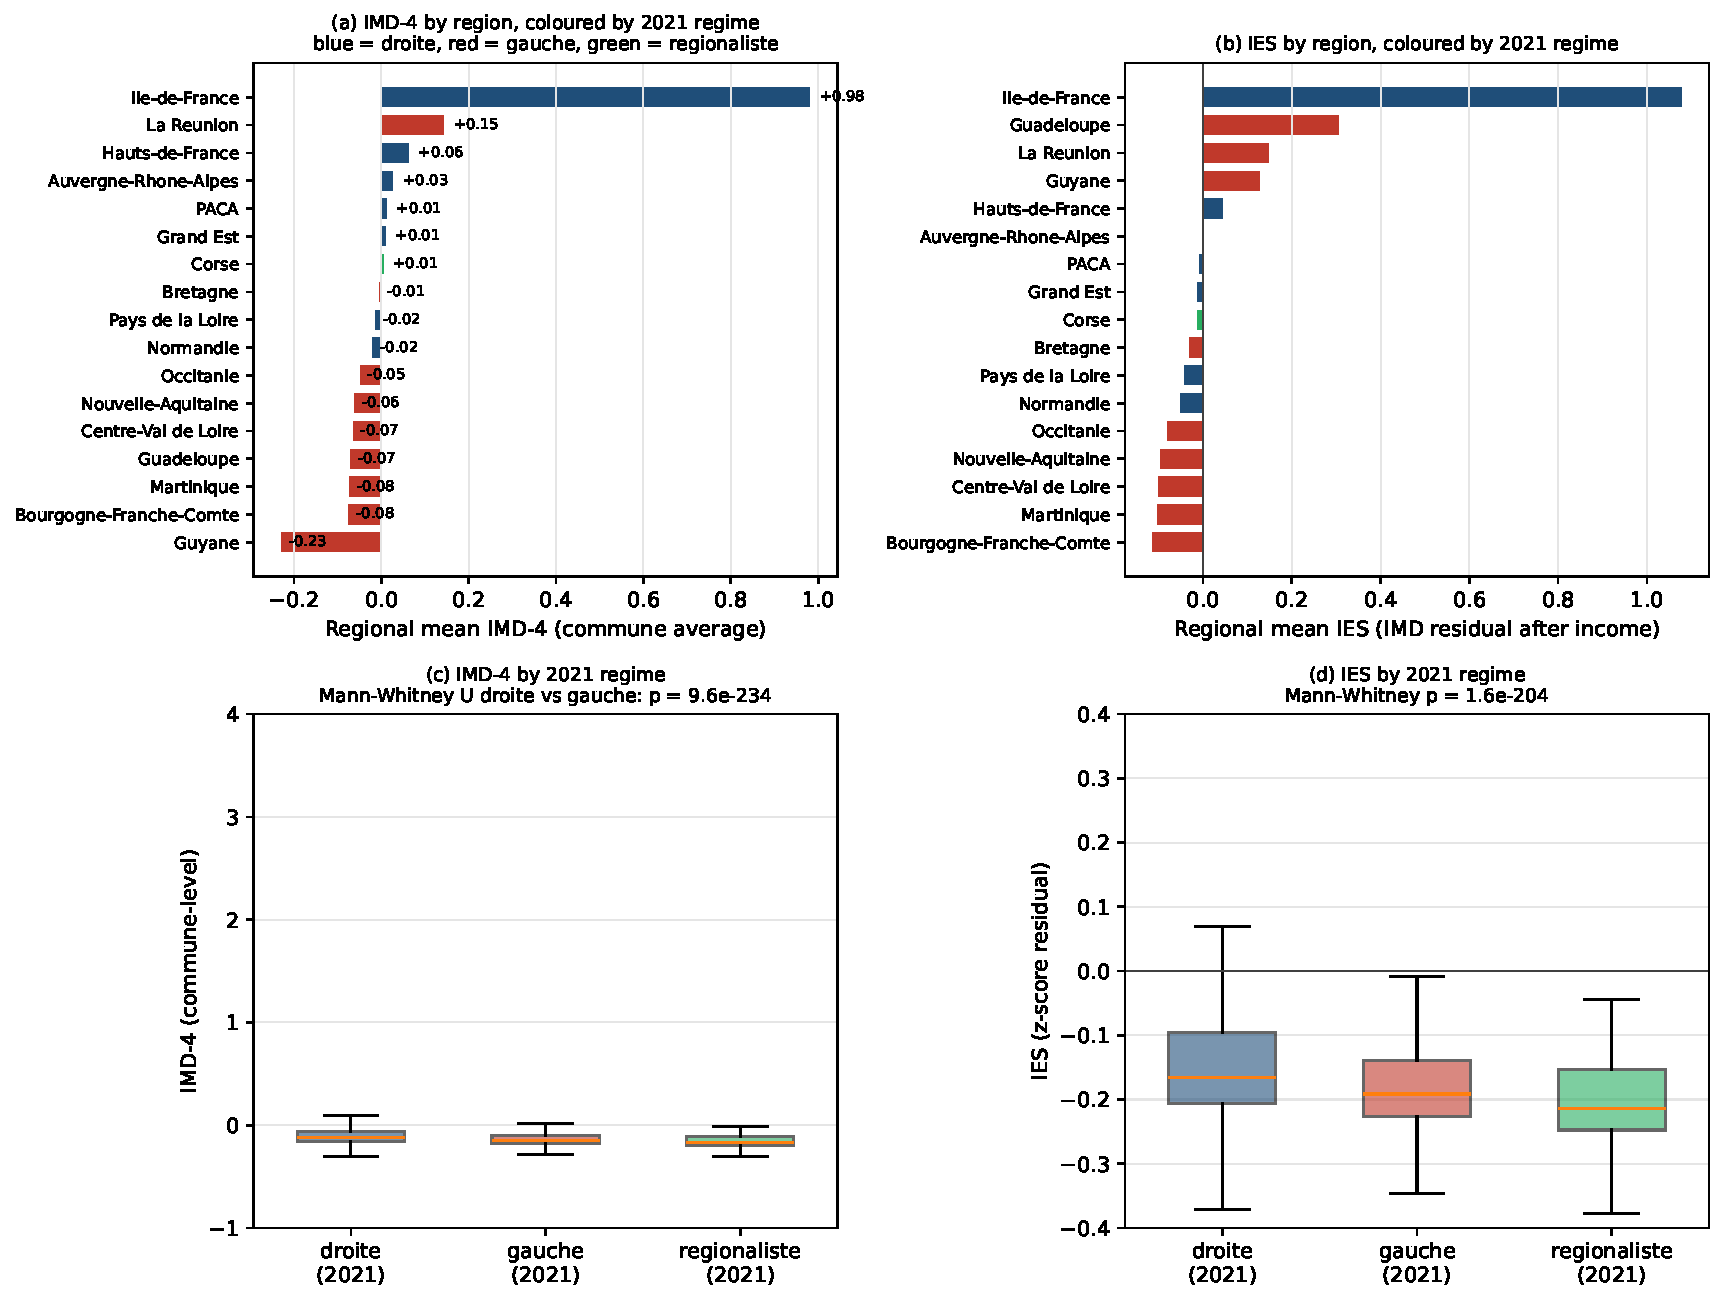
\includegraphics[width=0.99\linewidth]{b22_regional_political.pdf}
    \caption{Regional decomposition of the IMD-4 and IES by 2021
    political regime of the Conseil R\'egional.  (a)~Regional mean
    IMD-4 ; bar colour encodes the 2021 majority.  (b)~Regional
    mean IES.  (c-d)~Commune-level distributions by regime,
    boxplot (whiskers $1.5 \times$ IQR ; outliers hidden).  The
    apparent right-left gap in (c) is dominated by the
    \^Ile-de-France weight in the right aggregate.}
    \label{fig:regional}
\end{figure}

% =========================================================================
\section{Discussion}
\label{sec:discussion}

\subsection{What the IMD-4 is, and is not}

The IMD-4 is a \textbf{real-time, commune-resolution, public-data
composite indicator of cycling-environment quality}.  It is not a
measure of cycling \emph{behaviour} or \emph{perception} ; those
are the domains of EMP / recensement and FUB respectively, and the
IMD-4 is meant to complement them.  In particular, the IMD-4 is
explicitly \emph{supply-side} : it captures how good the cycling
context is, not how many people cycle.

Three implications follow.  First, the IMD-4 can be used as a
\emph{predictor} of cycling behaviour where direct observation is
unavailable -- e.g.\ between INSEE recensement waves (5-year
cycle) or in communes without an eco-counter ; the out-of-sample
$\rho = +0.42$ confirms this is feasible.  Second, the IMD-4 can
be used to \emph{flag potential targets} for Plan V\'elo
investment via the IES desert list of
Section~\ref{sec:ies}.  Third, the IMD-4 should \emph{not} be
used in isolation : a high IMD-4 indicates good cycling conditions
but does not guarantee high cycling use (\'Epinay-sur-Seine is a
clean false-positive example).

\subsection{Why the headline number is the residual gain over Cerema}

The single most important empirical finding of this paper is the
$+18$ percentage-point gain in $R^2$ on INSEE part-v\'elo-travail
that the IMD-4 obtains over Cerema infrastructure density alone
(Section~\ref{sec:residual}).  Cerema is the de facto national
standard for cycling-infrastructure monitoring ; that the IMD-4
adds meaningful explanatory power on top of it is the cleanest
defence of the multi-axis composition.  The four-component
specification is not just a re-packaging of Cerema -- it captures
cycling-environment signal that infrastructure km alone misses,
notably the multimodal context (M) and the demographic pool (D).

\subsection{Limits and follow-up work}

\textbf{Component T at national scale.}  The topographic component
is set to the panel z-score mean (zero) at national application
because BD ALTI 25\,m has not yet been integrated commune-by-commune.
The posterior weight on T is $0.08$, so the upper bound on the
information loss is $8\,\%$.  Adding national T is a follow-up
priority.

\textbf{Bus stops in M.}  Heavy-transit stops (train, m\'etro,
tramway) are the M numerator ; bus stops are excluded because they
do not generate the bike-and-ride dynamic at the same scale.  An
M' specification including high-frequency bus lines is a useful
sensitivity analysis.

\textbf{Causality.}  All correlations and regressions reported here
are cross-sectional.  A longitudinal IMD-4 panel -- which would
require recomputing the four components year-by-year on the same
communes -- would let us test whether an increase in cycling
infrastructure causes a shift in commune cycling commute share.
The data are public for all required inputs ; only the time-series
pipeline is missing.

\textbf{Outre-mer specificity.}  Six of the top 15 deserts are in
La R\'eunion.  The Outre-mer cycling-environment problem is
specific (tropical climate, mountainous terrain on R\'eunion
itself, weak transit) and deserves a dedicated regional study.

% =========================================================================
\section{Conclusion}
\label{sec:conclusion}

We introduced the IMD-4, the first commune-resolution, real-time,
public-data composite indicator of cycling-environment quality
for French communes.  It is validated against five independent
behavioural / outcome references, it adds $+18\,$pt $R^2$ over
the standard Cerema infrastructure indicator, it generalises
out-of-sample on cross-validation, and it extends to all
$34{,}858$ French communes with a national-panel correlation
that matches the calibration-panel result on the 42 largest
cities.

Used jointly with INSEE income and poverty data the IMD-4
delivers the first commune-resolution national cycling-equity
diagnostic, identifying $362$ ``double-penalty'' priority communes
that the Plan V\'elo could target.  The IMD-4 captures a
geographic-demographic gradient, not a partisan one : its variation
across regions is fully explained by density, urbanisation and
transit-stock heritage rather than the colour of the Conseil
R\'egional.

We release the full pipeline and per-commune IMD-4 and IES
tables under a permissive licence and welcome benchmarking against
future updates of FUB, EMP, eco-counter, BAAC, and INSEE recensement
data.

% =========================================================================
\appendix

\section{Tournament robustness}
\label{app:robust}

We summarise the bootstrap and leave-one-out diagnostics of the
five-reference tournament.  For every (metric, reference) cell we
compute a $1{,}000$-resample bootstrap $95\,\%$ CI on $\rho$ and a
leave-one-city-out range $[\rho_{\min}, \rho_{\max}]$ with the
most-influential city named.  The IMD-4 row is the only one in
which every CI strictly excludes zero.  The most-influential
city for the IMD-4 cells is most often Strasbourg, which is the
top-ranked metropole on three of the five references ; this is
the indicator's strength, not its fragility.

\bibliography{references}

\end{document}
